\section{CIFAR-10/100 Benchmarks with Fixed Training Cost}
\label{app:cifar_sc}
We also compared methods such that each took about the same cost on two virtual machines for 10,000 training samples (Figure \ref{fig:cifar_sc}). The baseline is RF's training times as run on the 2-core Standard\_DS2\_v2 Azure compute instance (Table \ref{table:azure}). 
% The SVM-RBF benchmarks were also run on the same compute instance for reference. 
As a result, the training wall times of CNNs, which often use the minimum epoch number, are always lower than those of RF. Due to the CNNs' different complexities, the correspondence between training costs becomes more accurate as the class number increases. The networks' training time trajectories also overlap more completely. The results are qualitatively similar to CIFAR benchmarks with fixed training time (Figure \ref{fig:cifar_st}).

\begin{figure}[!htb]
\centering
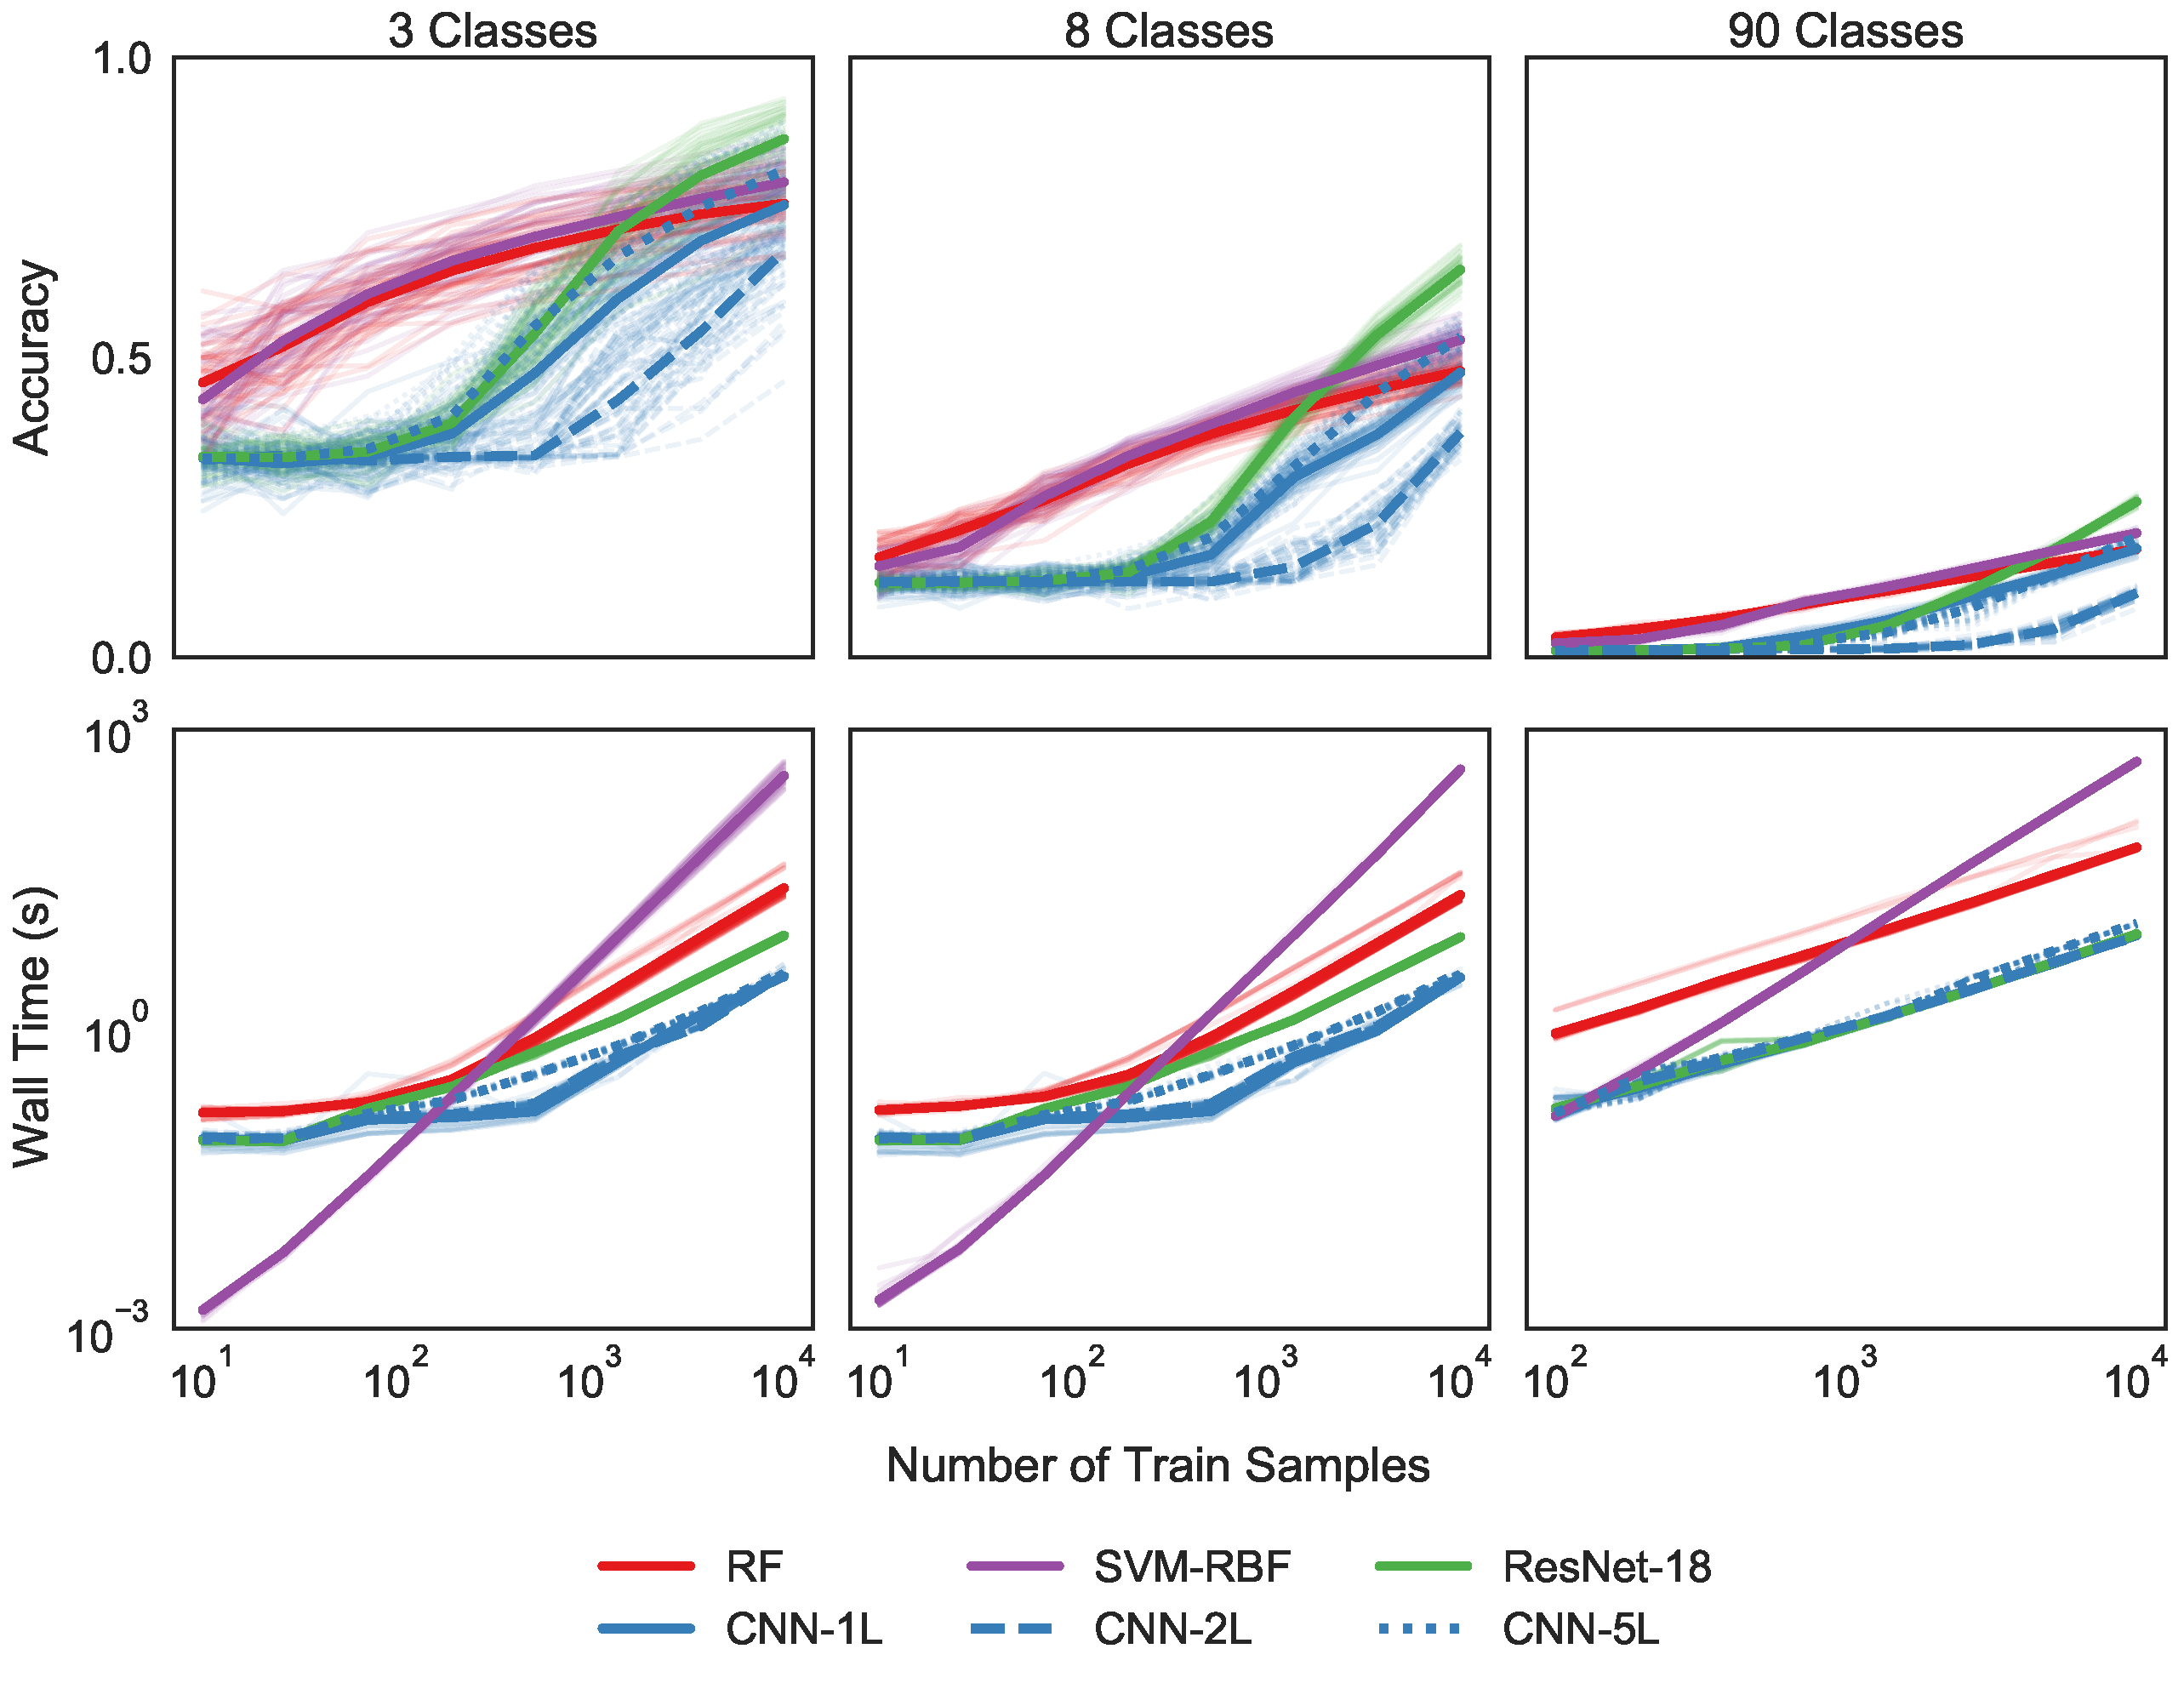
\includegraphics[width=0.8\textwidth]{figures/cifar_sc.pdf}
  \caption{Performance of forests and networks on multiclass CIFAR-10/100 classifications with fixed training cost.
  Upper row shows classifier accuracy on a linear scale, and bottom row shows training wall times in seconds on a logarithmic scale. The x-axes correspond to logarithmic sample sizes for respective columns. Each panel shows average results over 45 random combinations. The left two columns use CIFAR-10, while the rightmost uses CIFAR-100.
  RF has higher classification accuracy when compared to CNNs at smaller sample sizes. Complex networks, however, surpass RF at larger sample sizes, and ResNet-18 always performs best in the end.
  }
\label{fig:cifar_sc}
\end{figure}
\clearpage

\section{SVHN Benchmarks}
\label{app:svhn}
The SVHN dataset contains 73,257 digits for training and 26,032 for testing \citep{svhn}. The 3-class and 8-class tasks show surprising trends for networks, as simpler CNNs surpass ResNet-18 on classification accuracy as sample size increases. At higher sample sizes, 5-layer CNN has the best performance among all classifiers. Network accuracy is always higher than that of RF at 10,000 samples (Figure \ref{fig:svhn}). Although RF performs better than networks at smaller sample sizes in the 3-class task, the advantages disappear in the 8-class task. As seen in the CIFAR benchmarks (Figure \ref{fig:cifar}, \ref{fig:cifar_st}, \ref{fig:cifar_sc}), networks would be more adept at handling higher class numbers.

The trends of training wall times are very similar to those of CIFAR benchmarks with unbounded time and cost (Figure \ref{fig:cifar}). Forests' training times are always shorter than networks', and more fluctuations occur for CNN trajectories.

\begin{figure}[!htb]
\centering
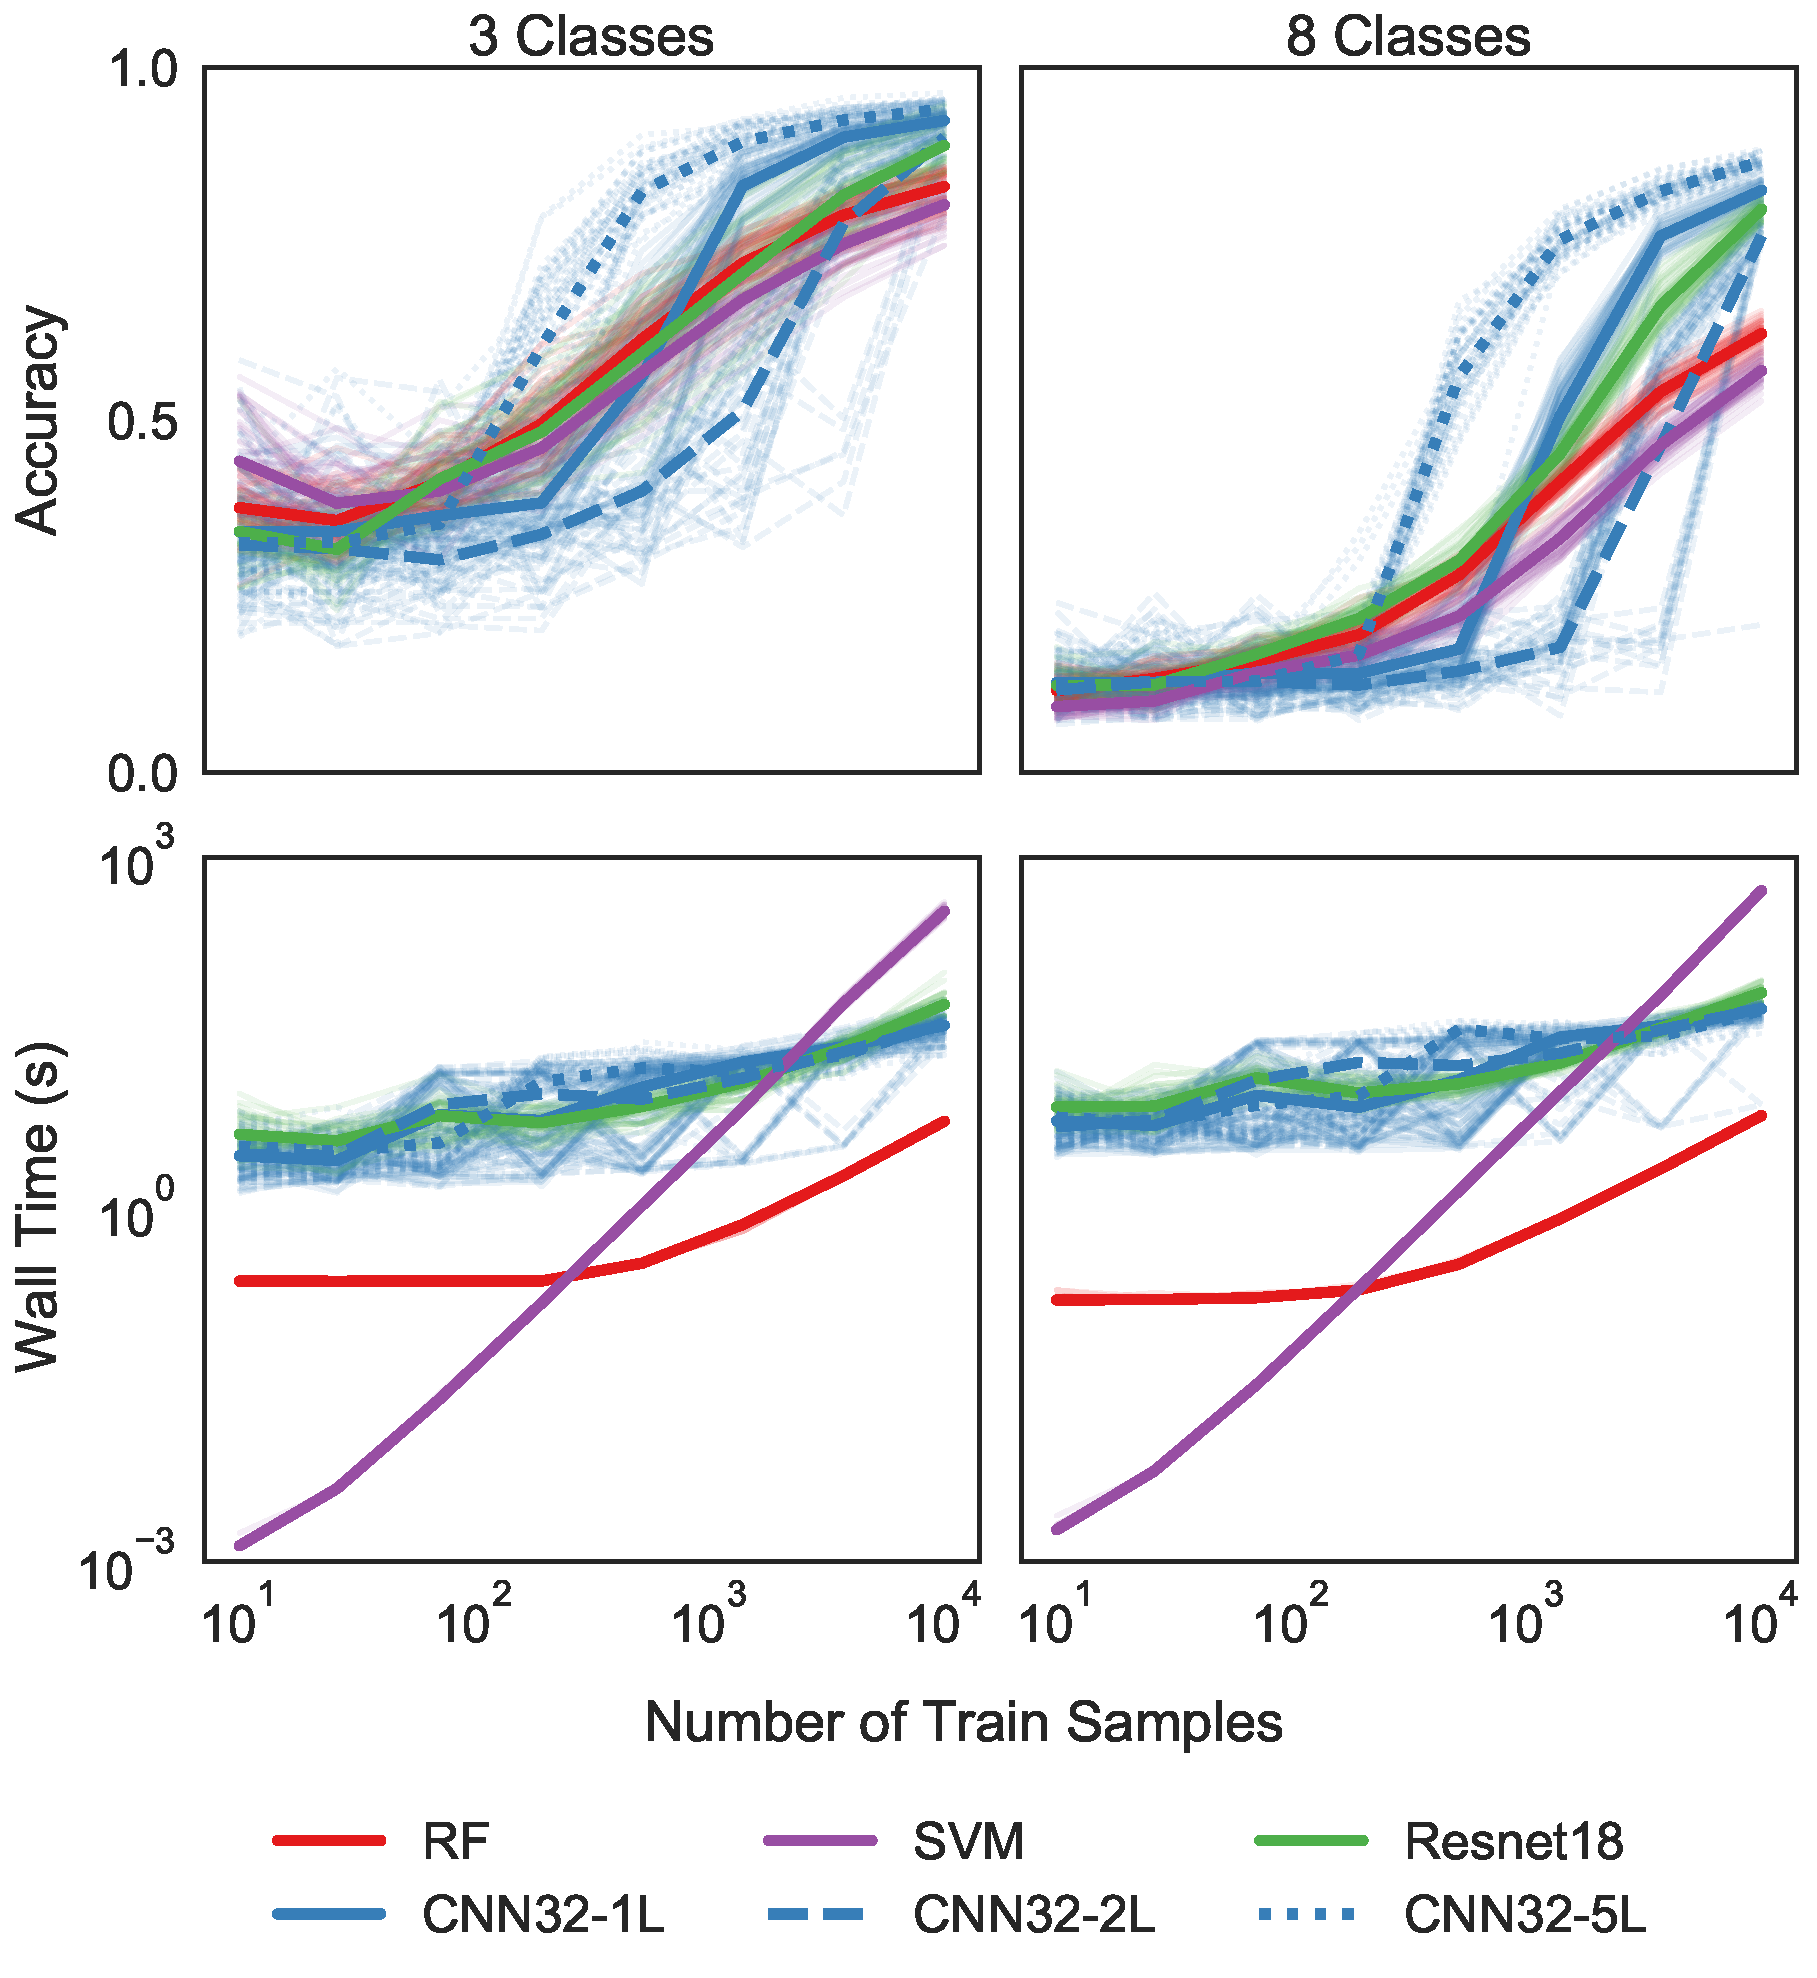
\includegraphics[width=0.6\textwidth]{figures/svhn.pdf}
  \caption{Performance of forests and networks on multiclass SVHN classifications with unbounded time and cost.
  Upper row shows classifier accuracy on a linear scale, and bottom row shows training wall times in seconds on a logarithmic scale. The x-axes correspond to logarithmic sample sizes for respective columns. Each column shows average results over 45 random combinations.
  Compared to CNNs, RF performs better and faster at smaller sample sizes.
  }
\label{fig:svhn}
\end{figure}
\clearpage

\section{FSDD Benchmarks with Mel-Spectrograms}
\label{app:mel}
As an alternative approach, we used PyTorch’s inbuilt function and converted the raw audio magnitudes into mel-spectrograms \citep{pytorch}. The process involves the aforementioned spectrogram conversions and uses triangular filterbanks to modify the images. The results (Figure \ref{fig:mel}) are qualitatively similar to FSDD benchmarks with spectrograms (Figure \ref{fig:spoken_digit}) and MFCCs (Figure \ref{fig:mfcc}).

\begin{figure}[!htb]
\centering
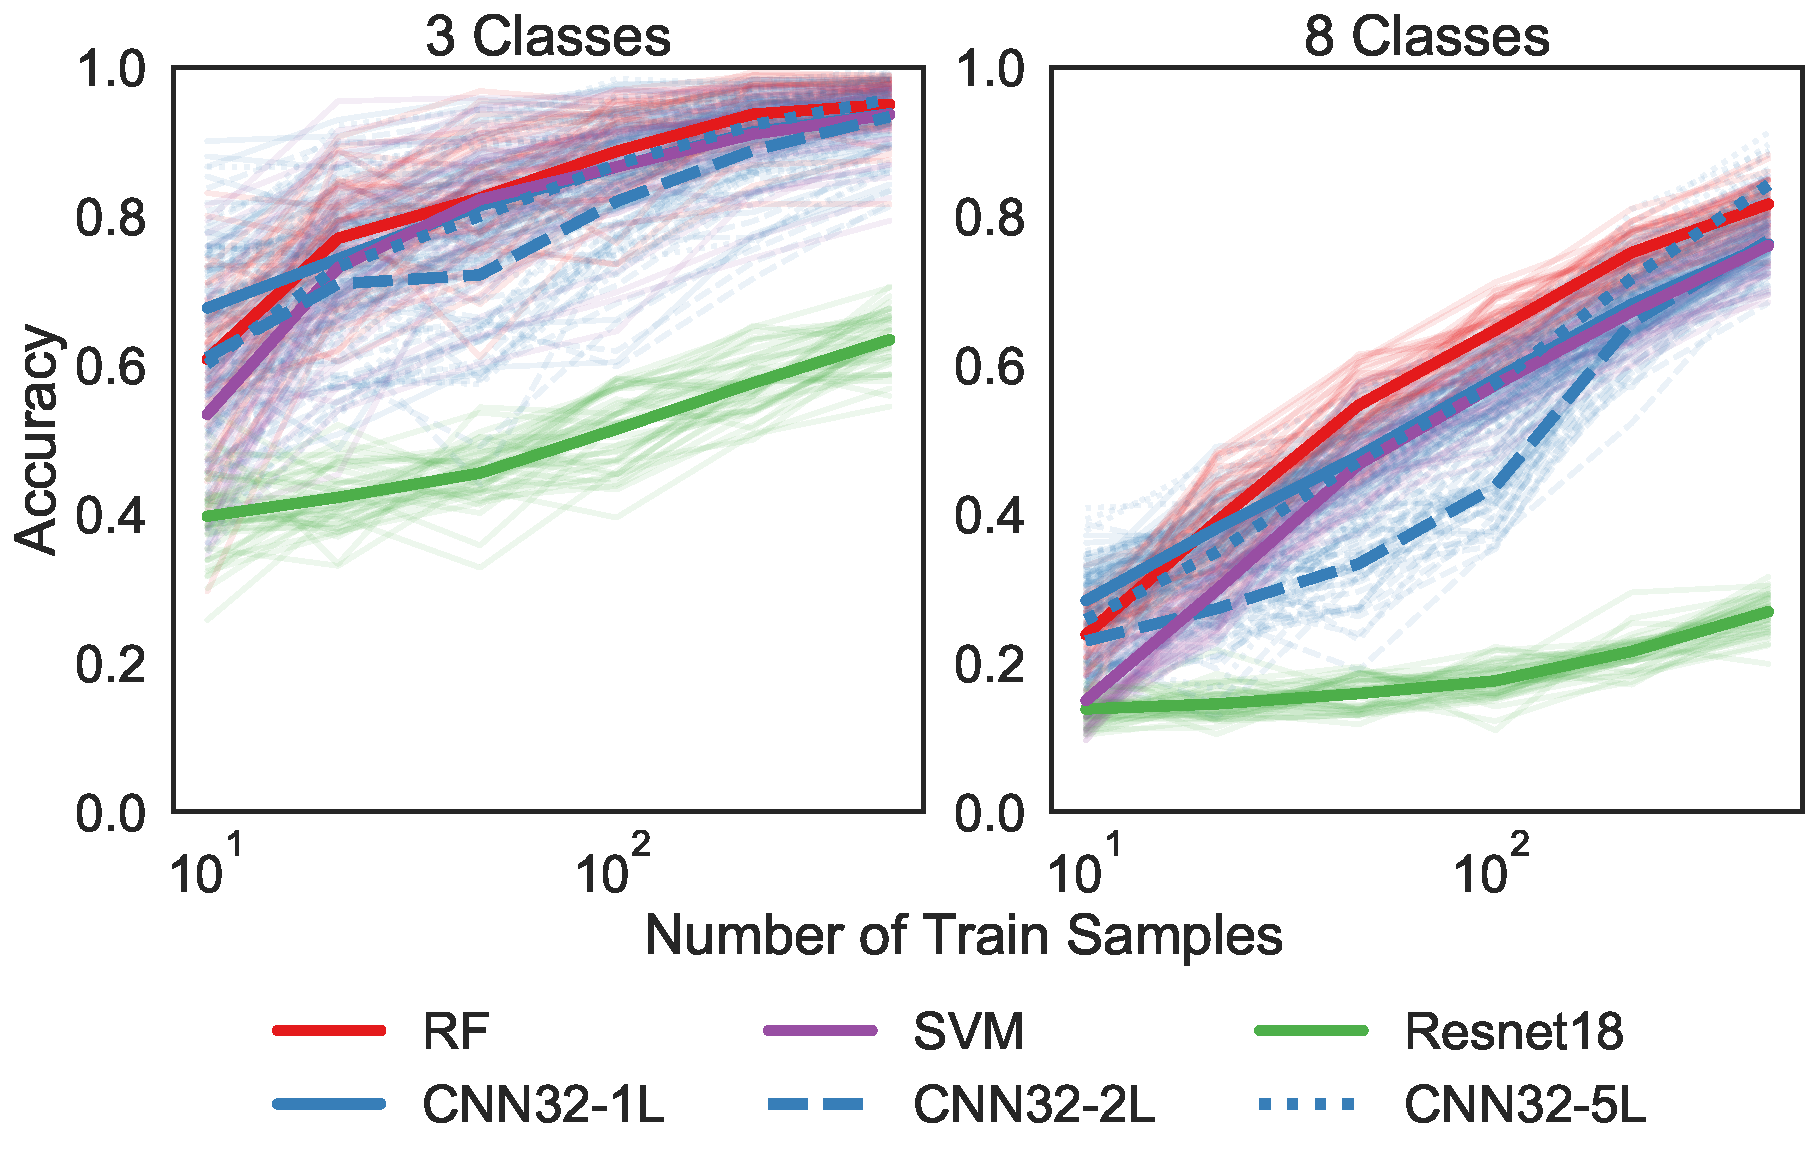
\includegraphics[width=0.6\textwidth]{figures/mel.pdf}
  \caption{Performance of forests and networks on multiclass FSDD classifications using mel-spectrograms.
  The y-axes represent classifier accuracy on a linear scale and the x-axes correspond to logarithmic sample sizes from 10 to 480. Each panel shows average results over 45 random class combinations and individual trajectories with lower alpha
  In the 3-class task, RF, 1-layer, and 5-layer CNNs all have very similar performances. In the 8-class task, RF achieves the highest accuracy. ResNet-18-Audio performs much worse than other classifiers.
  }
\label{fig:mel}
\end{figure}
\clearpage

\section{FSDD Benchmarks with MFCCs}
\label{app:mfcc}
As an alternative conversion, we used PyTorch’s inbuilt function and converted the raw audio magnitudes into MFCC \citep{pytorch}. The process calculates MFCCs on the DB-scaled mel-spectrograms. The results (Figure \ref{fig:mfcc}) are qualitatively similar to FSDD benchmarks with spectrograms (Figure \ref{fig:spoken_digit}) and mel-spectrograms (Figure \ref{fig:mel}).

\begin{figure}[!htb]
\centering
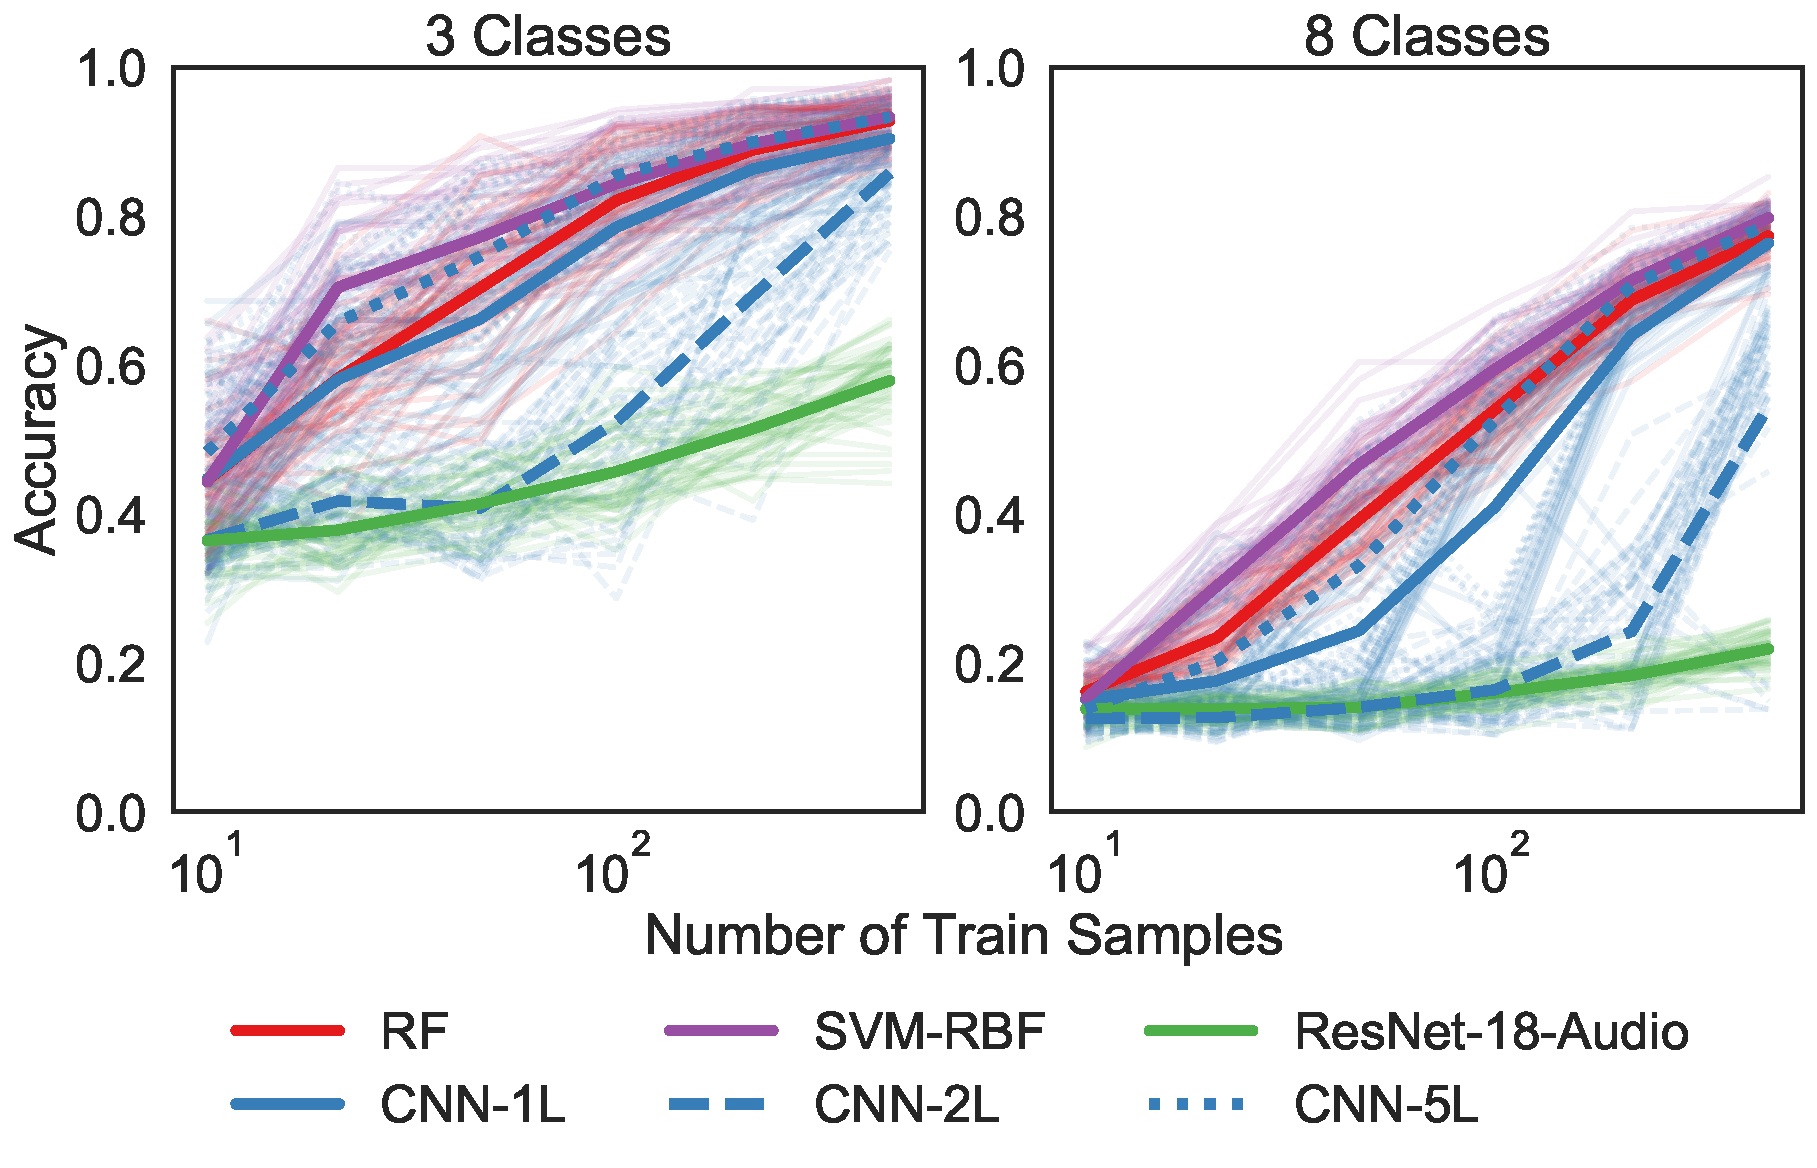
\includegraphics[width=0.6\textwidth]{figures/mfcc.pdf}
  \caption{Performance of forests and networks on multiclass FSDD classifications using mel-frequency cepstral coefficients (MFCC). 
  The y-axes represent classifier accuracy on a linear scale and the x-axes correspond to logarithmic sample sizes from 10 to 480. Each panel shows average results over 45 random class combinations and individual trajectories with lower alpha.
  At the maximum sample size, RF, 1-layer, and 5-layer CNNs all have very similar accuracy. 2-layer CNN performs worse, while ResNet-18-Audio performs the worst.
  }
\label{fig:mfcc}
\end{figure}
\clearpage

\section{Zebrafish Brain Maps}
\label{app:brains}
Figure \ref{fig:fluorian} illustrates neural selectivity to features of sensory input in a larval zebrafish, and indicates a learned partition and vote framework for brain functioning \citep{Naumann2016-oc}.
Specifically, this image shows all motion-sensitive nodes ($n = 76,604$) in a brain. Each node is a dot, color coded for preferred motion direction.
The image indicates that each node's activity indeed corresponds to a partition of feature space, which is actively refined through sensory experience and learning.
A relationship with forests and networks, at least at a basic level, is clear.
The utility of this relationship, for either machine learning or neuroscience, is the subject of endless conjecture and refutation.

\begin{figure}[h!]
\centering
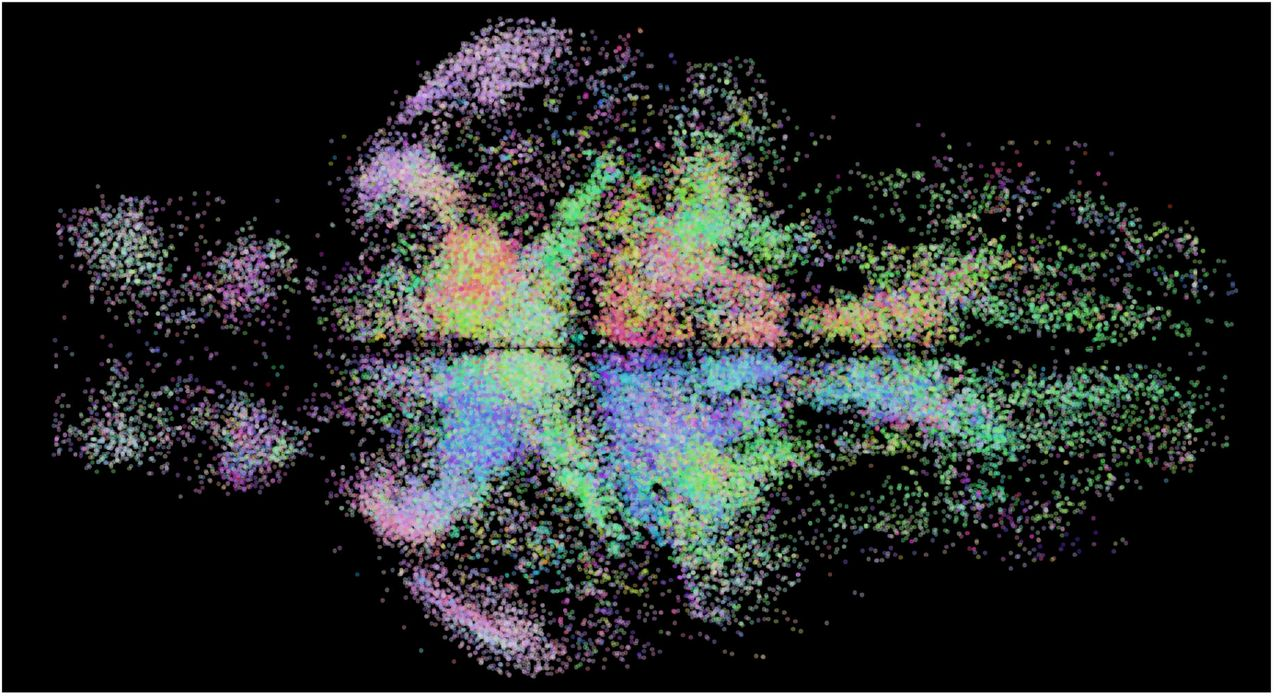
\includegraphics[width=0.7\textwidth]{figures/fish.jpg}
  \caption{Whole-brain activity maps reveal processing stages underlying the optomotor response in a larval zebrafish.
  }
\label{fig:fluorian}
\end{figure}
\clearpage
